% ============================================================
%  Chapter 5 — Pool-level valuation
%  Moved verbatim (June 2026 skeleton pass) from chapter4.tex §4.3:
%  the "from loans to pools" roll-forward results + economic
%  translation (Phase 3, M13–M15). The two former subsections are
%  promoted to sections §5.1/§5.2; the §4.3 lead paragraph now opens
%  the chapter. The four Phase-3 artifacts are F4.1 (fig:poolscatter),
%  T4.2 (tab:poolaccuracy), T5.1 (tab:econerrors), and F5.2
%  (fig:pricerrorbuckets); .tex tables regenerate via
%  dev/model/make_pool_tex.py from the committed M14/M15b JSON. All
%  numbers/tables/figures trace to outputs/{tables,figures}/pool_level.
% ============================================================

\chapter{Pool-level valuation}
\label{chap:poollevel}

The loan-level models of Section~\ref{sec:results-rolling} are now
aggregated to pools by the roll-forward of
Section~\ref{subsec:meth-pools}: for every loan alive at a window
anchor $t_0{=}\text{Dec}(k{-}1)$, the window-$k$ model's monthly
transition matrices are composed twelve steps forward to a horizon
event probability, and pool counts and speed paths follow from
\eqref{eq:poolcount} and Section~\ref{subsec:meth-econ}.  Only the
deterministic covariates evolve along the chain (loan age, remaining
term, calendar seasonality); the entire macroeconomic block --- rate
incentive, unemployment, house-price growth --- is \emph{frozen at the
anchor}, so every prediction is conditional on the $t_0$ environment.
Five regime-spanning anchors are scored, each with its own frozen
window-$k$ models: Dec2014 (calm), Dec2018 (late cycle), Dec2019
(entering the COVID forbearance shock), Dec2022 (the rate spike), and
Dec2024.

\section{Pool-level accuracy and the regime exhibit}

Figure~\ref{fig:poolscatter} is the flagship pool exhibit:
predicted versus realised twelve-month prepayment counts for the 500
random pools at Dec2024, one panel per model.  The improvement in
\emph{level} is stark --- the covariate-free empirical matrix predicts
roughly $2.5\times$ too many prepayments (its flat CPR floor ignores
that the 2024 cohort is deeply out of the money), the logit closes most
of the gap, and the ensemble cloud sits nearest the diagonal (RMSE
$82.9 \to 28.0 \to 11.9$ loans).  The $R^2$ values are all negative
even for the ensemble: random pools are near-homogeneous $1{,}000$-loan
draws, so cross-pool realised variance is tiny and $R^2$ is dominated
by a small level bias --- the random scheme tests \emph{level}
calibration, not cross-pool discrimination, which is why the
discriminating metric is read from the characteristic buckets instead.

Table~\ref{tab:poolaccuracy} gives that characteristic-bucket panel ---
$R^2$ and RMSE by model, outcome, and anchor --- and it is the regime
exhibit promised in Section~\ref{sec:intro-contributions}: a time
series of the value of nonlinearity, not a single verdict.
\textbf{Which model prices a pool best depends on whether the shock
lands in a covariate-captured channel.}  In calm and late-cycle
regimes the covariate models dominate (Dec2014 prepaid $R^2$
$0.58/0.98/0.98$ for empirical/logit/ensemble).  Under the
\emph{rate/prepayment-incentive shock} of 2022--24 --- precisely the
channel the rate-incentive covariates encode --- the empirical matrix
collapses to large negative $R^2$ ($-4.62$ at Dec2022, $-1.46$ at
Dec2024) while the ensemble is strongest ($0.85$, $0.94$; RMSE $415$
against the logit's $991$ at Dec2024).  But under the 2020
\emph{forbearance/credit shock} the ordering \emph{inverts}: at Dec2019
the assumption-free empirical floor is best ($R^2\,0.65$) and the
ensemble is worst ($0.45$), because the ensemble bakes in hardest a
pre-COVID prepayment signal that March 2020 abruptly invalidates.  For
the rare serious-delinquency outcome RMSE is the reliable metric (with
$\sim$16 buckets $R^2$ is unstable across all models), and the ensemble
is the only model with positive $60{+}$\,DPD $R^2$ at the 2022 and 2024
anchors.

\begin{figure}[htbp]\centering
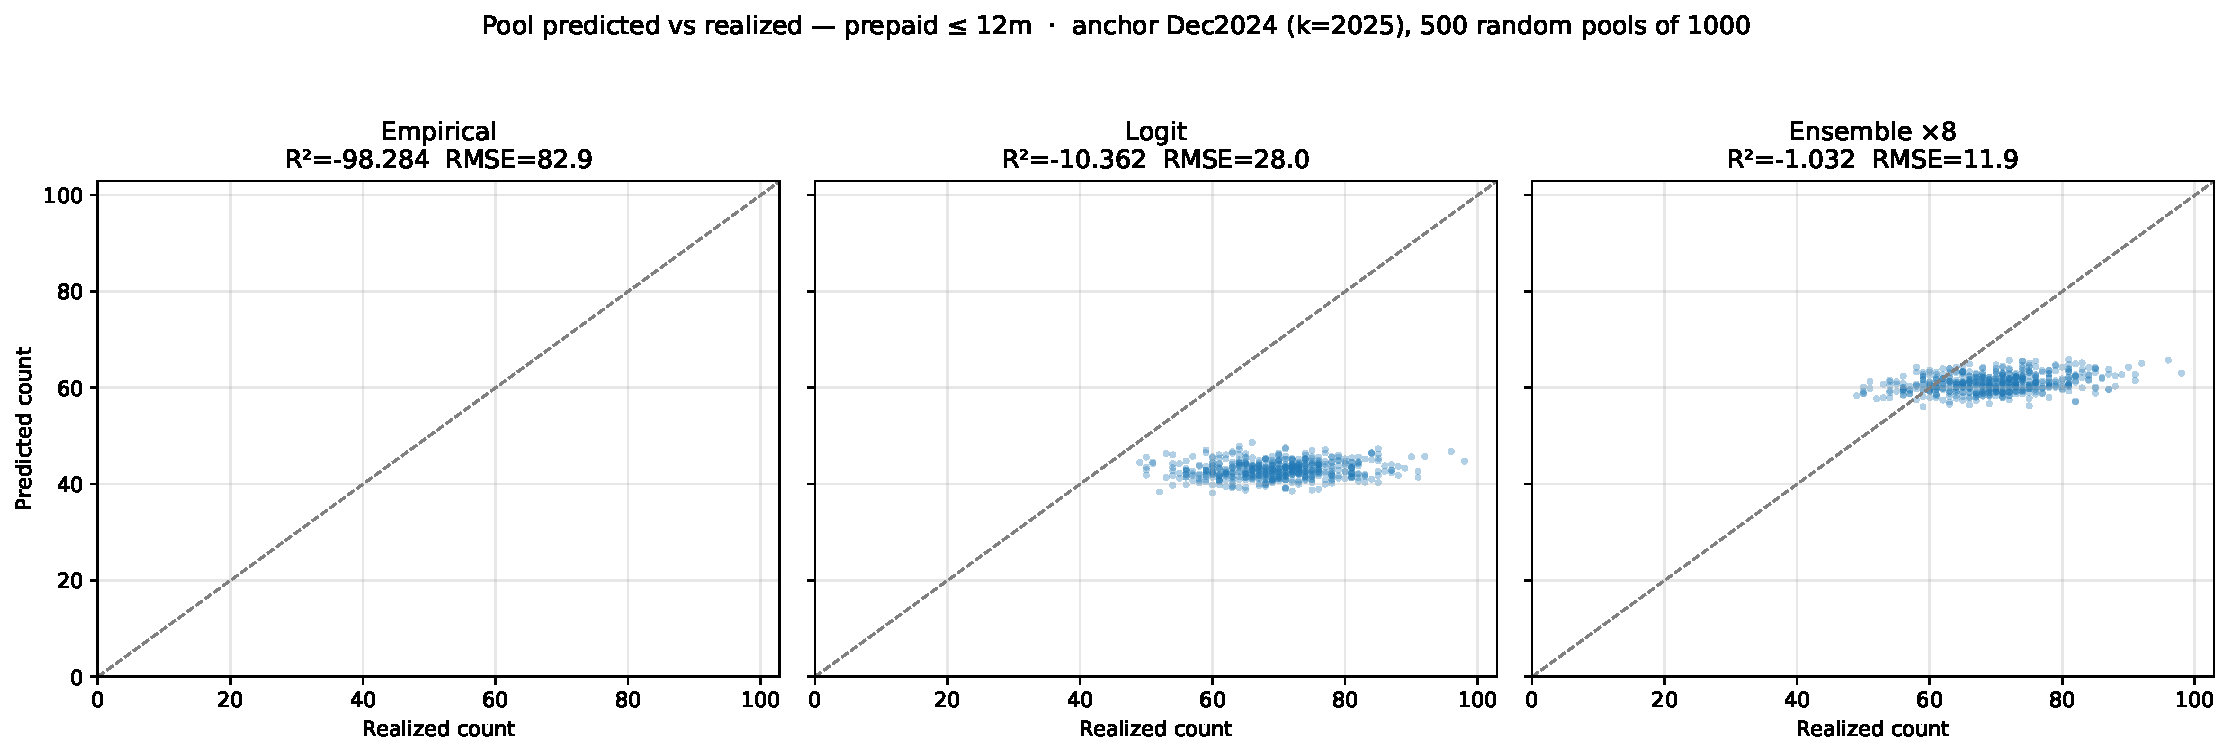
\includegraphics[width=0.95\textwidth]{figs/F4.1_scatter_random_prepaid.pdf}
\caption[Predicted versus realised pool prepayment counts, random
pools]{Predicted versus realised twelve-month prepayment counts, 500
random pools of 1{,}000 loans at the Dec2024 anchor, by model.  The
dashed line is $45^\circ$.  Level calibration improves
empirical\,$\to$\,logit\,$\to$\,ensemble (RMSE $82.9/28.0/11.9$);
$R^2$ is uninformative for homogeneous random pools (see
text).}\label{fig:poolscatter}
\end{figure}

\begin{table}[htbp]\centering\small
\caption[Characteristic-bucket pool accuracy by model, outcome, and
anchor]{Pool-level $R^2$ and RMSE on the characteristic buckets
(credit$\,\times\,$rate$\,\times\,$LTV cells, $\geq2{,}000$ loans each)
by model, outcome, and anchor.  The interpretable cross-pool panel;
random-pool $R^2$ is discussed in the text.  RMSE is in loans.  Shock-type
dependence: covariate models dominate off-COVID and under the rate
shock, but the empirical floor is most robust at the 2020 forbearance
break.}\label{tab:poolaccuracy}
% Source: outputs/tables/pool_level/t_m14_pool_counts.json (M14, full run).
% Characteristic-bucket panel (FICO x orig-rate-quartile x LTV, >=2000 loans/cell): the
% interpretable cross-pool metric. Random-pool R^2 is uninformative by construction
% (homogeneous ~1000-loan draws) and is discussed in text, not tabulated. For the rare
% 60+ DPD outcome read RMSE, not R^2 (>=~16 buckets makes R^2 unstable). Caption in chapter4.tex.
\begin{tabular}{llrrrrrr}
\toprule
 & & \multicolumn{3}{c}{$R^2$} & \multicolumn{3}{c}{RMSE (loans)} \\
\cmidrule(lr){3-5}\cmidrule(lr){6-8}
Outcome & Anchor & Emp. & Logit & Ens. & Emp. & Logit & Ens. \\
\midrule
\multirow{5}{*}{Prepaid} & Dec2014 & 0.575 & 0.980 & 0.981 & 1517 & 328 & 320 \\
 & Dec2018 & 0.744 & 0.607 & 0.791 & 1118 & 1387 & 1011 \\
 & Dec2019 & 0.647 & 0.537 & 0.449 & 3054 & 3500 & 3817 \\
 & Dec2022 & -4.616 & 0.742 & 0.848 & 3303 & 708 & 542 \\
 & Dec2024 & -1.455 & 0.651 & 0.939 & 2627 & 991 & 415 \\
\midrule
\multirow{5}{*}{60+ DPD} & Dec2014 & -4.525 & -0.782 & 0.299 & 449 & 255 & 160 \\
 & Dec2018 & -8.699 & -1.230 & -0.390 & 423 & 203 & 160 \\
 & Dec2019 & -0.165 & -0.467 & -0.464 & 591 & 663 & 663 \\
 & Dec2022 & -17.181 & -0.155 & 0.635 & 514 & 129 & 73 \\
 & Dec2024 & -16.461 & -0.063 & 0.261 & 471 & 116 & 97 \\
\bottomrule
\end{tabular}

\end{table}

\section{Economic translation: speed, timing, and price errors}

Restating these count comparisons in valuation units
(Section~\ref{subsec:meth-econ}) sharpens the contribution.
Table~\ref{tab:econerrors} reports mean absolute speed (CPR), timing
(weighted-average life), and price errors on the characteristic
buckets, with the ensemble-versus-logit reduction in the last column;
all errors are model-implied minus realised-speed valuation through the
same engine, so the price column isolates the prepayment forecast.  The
headline is the price row, \textbf{reported per anchor because it
inverts at COVID and a pooled average would conceal that}: the ensemble
cuts the logit's mean absolute price error by $+18\%$ at Dec2014
($0.148\to0.121$ per 100 face), $+25\%$ at Dec2018
($0.560\to0.418$), $+31\%$ at Dec2022 ($0.254\to0.176$), and $+48\%$ at
Dec2024 ($0.233\to0.122$), but by $-1\%$ at the Dec2019 COVID anchor
($0.583\to0.587$) --- the same inversion as the counts, now in price.
The absolute magnitudes are economically modest in aggregate (fractions
of a point per 100 of face), as expected when the discount curve is
fixed and the pools diversify idiosyncratic timing; the action is in
\emph{where} the error concentrates.

Figure~\ref{fig:pricerrorbuckets} maps the signed price error across
credit\,$\times$\,rate cells at the Dec2022 rate-spike anchor, per
model.  The empirical matrix misprices everywhere ($-0.7$ to $-1.2$ per
100, over-predicting prepayment uniformly).  The logit's error is
benign in the low-rate cells but \textbf{concentrates in the
high-incentive top rate quartile} --- $-0.35$ to $-0.61$ per 100, where
its linear-in-incentive form over-fires prepayment on high-coupon loans
whose incentive had in fact collapsed after the 2022 rate rise.  The
ensemble compresses exactly those cells to $-0.15$ to $-0.32$.  This is
the pricing mirror of the prepayment S-curve of
Section~\ref{subsec:data-eda-single}: the linear model breaks where the
hazard is most curved, and that is where dollars of mispricing collect.

\begin{table}[htbp]\centering\small
\caption[Pool CPR, weighted-average-life, and price errors by model and
anchor]{Mean absolute CPR (percentage points), weighted-average-life
(months), and price (per 100 face) error on the characteristic buckets,
by model and anchor, with the ensemble-versus-logit reduction.  Errors
are model-implied minus realised-speed valuation through the same
level-pay engine and discount curve.  The price row is the headline;
reported per anchor because the 2020 anchor
inverts.}\label{tab:econerrors}
% Source: outputs/tables/pool_level/t_m15_econ_errors.json (M15b).
% Characteristic-bucket panel. Each model cell is the mean |error| over the bucket pools;
% errors = model-implied minus realized-SMM valuation through the same level-pay engine
% (identical WAC/WAM/UPB, WAC-25bp curve, so price dispersion isolates the prepay model).
% Last column = ensemble-vs-logit reduction in that row's mean |error| (the price row is the
% headline). Reported per anchor, never pooled (the Dec2019 COVID anchor inverts). Caption in chapter4.tex.
\begin{tabular}{llrrrr}
\toprule
Metric & Anchor & Empirical & Logit & Ensemble & Ens.\,vs\,Logit \\
\midrule
\multirow{5}{*}{\shortstack[l]{Price error\\(per 100 face)}} & Dec2014 & 0.228 & 0.148 & 0.121 & $+18\%$ \\
 & Dec2018 & 0.205 & 0.560 & 0.418 & $+25\%$ \\
 & Dec2019 & 0.552 & 0.583 & 0.587 & $-1\%$ \\
 & Dec2022 & 1.068 & 0.254 & 0.176 & $+31\%$ \\
 & Dec2024 & 0.657 & 0.233 & 0.122 & $+48\%$ \\
\midrule
\multirow{5}{*}{\shortstack[l]{CPR error\\(pp)}} & Dec2014 & 4.30 & 2.34 & 3.28 & $-40\%$ \\
 & Dec2018 & 3.14 & 6.28 & 4.79 & $+24\%$ \\
 & Dec2019 & 17.08 & 16.69 & 17.41 & $-4\%$ \\
 & Dec2022 & 11.80 & 2.69 & 1.56 & $+42\%$ \\
 & Dec2024 & 9.30 & 2.02 & 0.50 & $+75\%$ \\
\midrule
\multirow{5}{*}{\shortstack[l]{WAL error\\(months)}} & Dec2014 & 14.8 & 10.1 & 8.1 & $+20\%$ \\
 & Dec2018 & 13.3 & 38.5 & 28.5 & $+26\%$ \\
 & Dec2019 & 34.0 & 35.7 & 35.8 & $0\%$ \\
 & Dec2022 & 72.0 & 18.9 & 12.9 & $+32\%$ \\
 & Dec2024 & 42.6 & 16.2 & 9.3 & $+43\%$ \\
\bottomrule
\end{tabular}

\end{table}

\begin{figure}[htbp]\centering
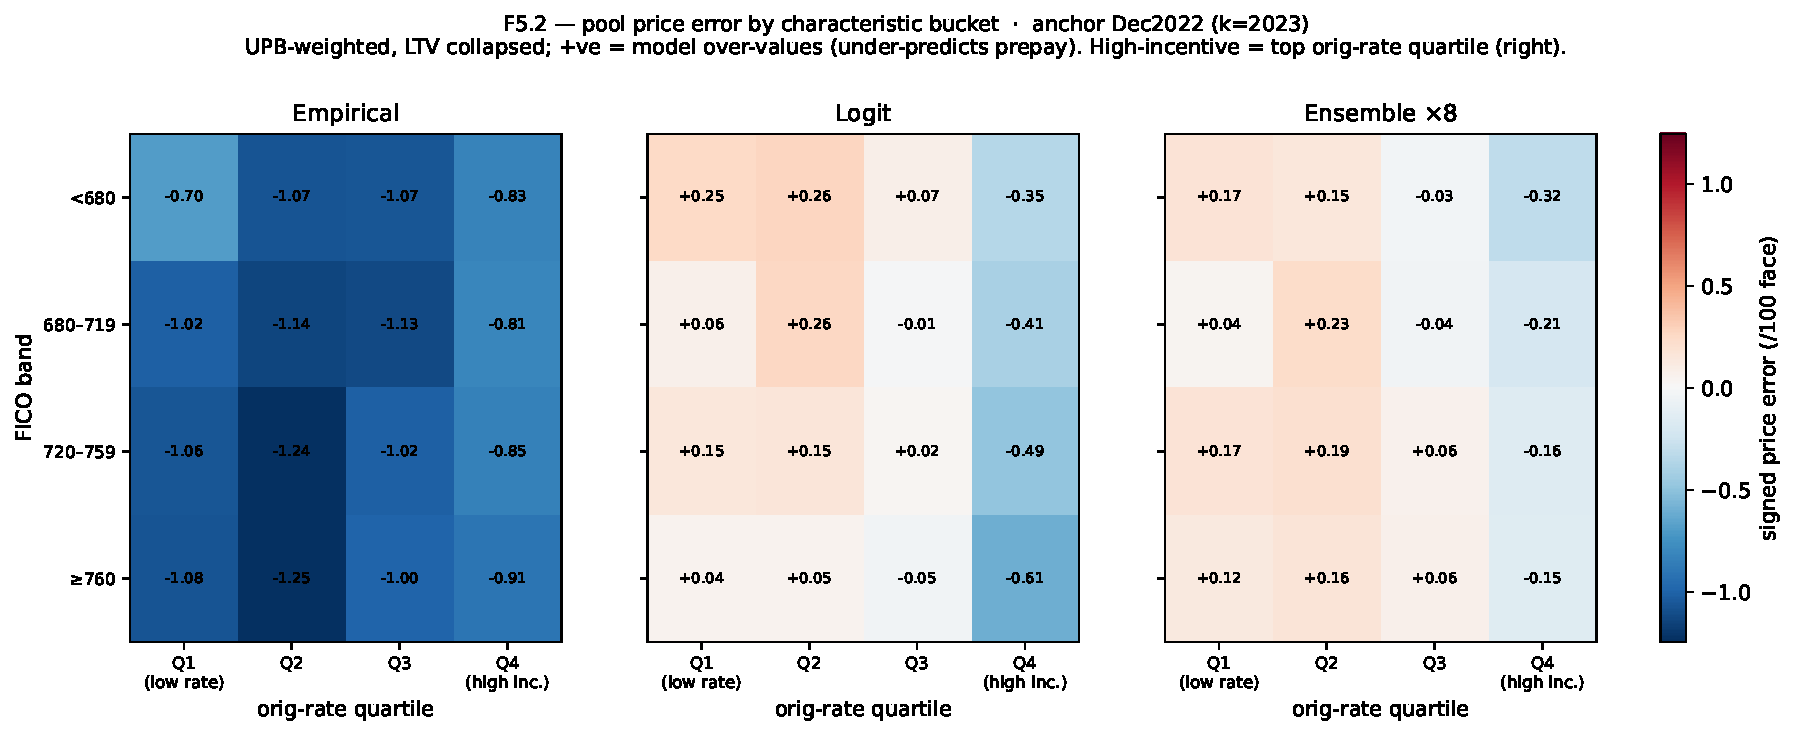
\includegraphics[width=0.95\textwidth]{figs/F5.2_price_error_buckets.pdf}
\caption[Pool price error by characteristic bucket and model]{Signed
price error (per 100 face, UPB-weighted, LTV collapsed) by
credit\,$\times$\,original-rate-quartile cell at the Dec2022 anchor, per
model; positive means the model over-values the pool by under-predicting
prepayment.  The logit's error concentrates in the high-incentive top
rate quartile (right column), which the ensemble
compresses.}\label{fig:pricerrorbuckets}
\end{figure}

\paragraph{Why price is not simply average CPR.}  A pool's price
depends on the \emph{timing} of returned principal --- the full monthly
speed path and hence the weighted-average life --- not on the average
speed alone, which is what makes the cashflow engine more than a
relabelling of CPR.  The two can even rank models differently: at
Dec2014 the logit's mean CPR error is the smaller ($2.34$ against the
ensemble's $3.28$ percentage points), yet the ensemble still prices the
buckets better ($+18\%$ lower price error), because it places its
prepayments at more accurate \emph{months}.  Reassuringly, the engine
is internally coherent --- across all pools and anchors the sign of the
price error agrees with the sign of the weighted-average-life error in
$99.4$--$100\%$ of cases (slower prepayment $\Rightarrow$ longer life
$\Rightarrow$ higher price on these premium pass-throughs).  The
price-versus-CPR sign disagreements occur \emph{only} where the CPR
error is itself negligible (median $0.5$--$1.6$ against $2$--$4.5$
percentage points where they agree): when average speeds nearly match,
timing is what remains, and only the price and life errors can see it.

\paragraph{The frozen-anchor caveat.}  These are
\emph{prepayment-model} valuation errors at a fixed discount curve with
the macroeconomic environment frozen at each anchor, not full
option-adjusted spreads (Section~\ref{subsec:meth-econ}).  The
single regime where this assumption bites hardest is the one it is
designed to expose: at Dec2019 every model under-predicts the realised
$33\%$ CPR by about seventeen percentage points, because all are blind
to the March-2020 rate collapse and refinancing wave that no $t_0$
covariate could anticipate.  Far from a flaw, this is the cleanest
statement of the design's boundary --- it prices the prepayment model,
holding the world fixed --- and it is exactly why the value of
nonlinearity must be read as regime-conditional rather than as a single
headline number.
